%Master File:lectures.tex


\lesson{Support Vector Machines}
\vspace{-2cm}
\begin{center}
  \includegraphics[height=11cm]{svm-data1}
\end{center}
\keywords{Support Vector Machines, maximum margins}
%%%%%%%%%%%%%%%%%%%%%%% Next Slide %%%%%%%%%%%%%%%%%%%%%%%
\renewcommand{\Outline}{%
\begin{slide}
\section[1]{Outline}

\begin{minipage}{8cm}\raggedright
  \begin{enumerate}
    \outlineitem{The Big Picture}{svmover}
    \outlineitem{Maximum Margins}{maxmargin}
    \outlineitem{Duality}{duality}
    \outlineitem{Practice}{practice}
  \end{enumerate}
\end{minipage}\hfill
\begin{minipage}{15cm}
  \includegraphics[width=15cm]{svm-data1}
\end{minipage}
\end{slide}
\addtocounter{outlineitem}{1}
}

\setcounter{outlineitem}{1}

%%%%%%%%%%%%%%%%%%%%%%% Next Slide %%%%%%%%%%%%%%%%%%%%%%%
\Outline % Overview
\toptarget{firstoutline}
%%%%%%%%%%%%%%%%%%%%%%% Next Slide %%%%%%%%%%%%%%%%%%%%%%%

\begin{slide}
\section{Support Vector Machines}

\begin{PauseHighLight}
  \begin{itemize}
  \item Support vector machines, when used right, often have the best
    generalisation results\pause
  \item They are typically used on numerical data, but can and have been
    adapted to text, sequences, etc.\pause
  \item Although not as trendy as deep learning, they will often be the
    method of choice on small data sets\pause
  \item They subtly regularise themselves, choosing a solution that
    generalises well from a host of different solutions\pause
  \end{itemize}
\end{PauseHighLight}

\end{slide}


%%%%%%%%%%%%%%%%%%%%%%% Next Slide %%%%%%%%%%%%%%%%%%%%%%%

\begin{slide}
\section[-2]{Linear Separation of Data}

\pb
\begin{itemize}
\item SVMs classify linearly separable data\pause\pauselevel{=1}
  \begin{center}
    \multipdf[width=0.8\linewidth]{maxMargin}\pause
  \end{center}
\item Finds maximum-margin separating plane\pauseb
\end{itemize}

\end{slide}

%%%%%%%%%%%%%%%%%%%%%%% Next Slide %%%%%%%%%%%%%%%%%%%%%%%

\begin{slide}
\section[-2]{Extended Feature Space}

\begin{PauseHighLight}
  \begin{itemize}
  \item To increase the likelihood of linear-separability we often use a
    high-dimensional mapping
    \begin{align*}
      \bm{x}=(x_1,\,x_2,\,\ldots,\,x_p)^\tr \rightarrow \bm{\phi}(\bm{x}) =
      (\phi_1(\bm{x}),\,\phi_2(\bm{x}),\,\ldots,\,
      \phi_r(\bm{x}))^\tr
    \end{align*}
    $r\gg p$\pause
  \item Finding the maximum margin hyper-plane is time consuming in
    ``primal'' form if $r$ is large\pause
  \item We can work in the ``dual'' space of patterns, then we only need to
    compute inner-products
    \begin{align*}
      \langle \bm{\phi}(\bm{x}_i), \bm{\phi}(\bm{x}_j) \rangle =
      \bm{\phi}(\bm{x}_i)^\tr \bm{\phi}(\bm{x}_j)  \pause
      =  \sum_{k=1}^r \phi_k(\bm{x}_i) \, \phi_k(\bm{x}_j)\pauseb
    \end{align*}
  \end{itemize}
\end{PauseHighLight}

\end{slide}

%%%%%%%%%%%%%%%%%%%%%%% Next Slide %%%%%%%%%%%%%%%%%%%%%%%

\begin{slide}
\section[-1]{Kernel Trick}

\begin{PauseHighLight}
  \begin{itemize}
  \item If we choose a \emph{positive semi-definite} kernel function
    $K(\bm{x}, \bm{y})$ then there exists functions
    $\bm{\phi}(\bm{x}) = (\phi_k(\bm{x})|k=1,\,2,\,\ldots,\,r)$,
    such that
    \begin{align*}
      K(\bm{x}_i, \bm{x}_j) = \bm{\phi}(\bm{x}_i)^\tr
      \bm{\phi}(\bm{x}_j) \pause
    \end{align*}
    (like an eigenvector decomposition of a matrix)\pause
  \item Never need to compute $\phi_k(\bm{x}_i)$ explicitly as we only
    need the inner-product $\bm{\phi}(\bm{x}_i)^\tr
      \bm{\phi}(\bm{x}_j) = K(\bm{x}_i, \bm{x}_j)$ to compute maximum
      margin separating hyper-plane\pause
    \item Sometimes $\bm{\phi}(\bm{x}_i)$ is an infinite dimensional
      vector so it is good we don't have to compute all the elements!\pause
  \end{itemize}
\end{PauseHighLight}

\end{slide}
%%%%%%%%%%%%%%%%%%%%%%% Next Slide %%%%%%%%%%%%%%%%%%%%%%%

\begin{slide}
\section[-2]{Kernel Functions}

\begin{PauseHighLight}
  \begin{itemize}
  \item Kernel functions are symmetric functions of two variable\pause
  \item Strong restriction: \textit{positive semi-definite}\pause
  \item Examples
    \begin{align*}
      \mbox{Quadratic kernel:}&& K(\bm{x}_1,\,\bm{x}_2)&=
      \left(\bm{x}_1^\tr\bm{x}_2\right)^2 \\
      \mbox{Gaussian (RBF) kernel:}&& K(\bm{x}_1,\,\bm{x}_2)&=
      \mathrm{e}^{-\gamma\,\|\bm{x}_1-\bm{x}_2\|^2}\pause
    \end{align*}
  \item Consider the mapping
    \begin{align*}
      \bm{x}_i =
      \begin{pmatrix}
        x_i \\ y_i
      \end{pmatrix}
      \rightarrow
      \bm{\phi}(\bm{x}_i) =
      \begin{pmatrix}
        x_i^2 \\ y_i^2 \\ \sqrt{2}\,x_i\,y_i 
      \end{pmatrix}\pause
    \end{align*}
  \end{itemize}
\end{PauseHighLight}

\end{slide}


%%%%%%%%%%%%%%%%%%%%%%% Next Slide %%%%%%%%%%%%%%%%%%%%%%%

\begin{slide}
\section[-3]{Non-linearly Separation of Data}
\toptarget{svm}
\pb
{\small
\begin{align*}
  K(\bm{x}_1,\,\bm{x}_2) &= 
\begin{pmatrix}
   x_1^2 & y_1^2 & \sqrt{2}\,x_1\,y_1
\end{pmatrix}
\begin{pmatrix}
  x_2^2 \\ y_2^2 \\ \sqrt{2}\,x_2\,y_2 
\end{pmatrix}\pause
=  x_1^2\,x_2^2 + y_1^2\,y_2^2 + 2 \,x_1\,y_1\,x_2\,y_2 \pause \\
&= (x_1\,x_2 + y_1\,y_2)^2 \pause =  \left(\bm{x}_1^T\bm{x}_2\right)^2\pause
\end{align*}}
\setlength{\unitlength}{\linewidth}
\begin{picture}(1,0.4)
\put(-0.02,0){\includegraphics[width=0.43\linewidth]{nonlinsep}}\pause
\put(0.42,0.18){$\stackrel{\bm{x}\rightarrow\bm{\phi}(\bm{x})}{\longrightarrow}$}\pause
\put(0.54,0){\includegraphics[width=0.51\linewidth]{svm-data0}}\pause
\put(0.54,0){\includegraphics[width=0.51\linewidth]{svm-data1}}\pause
\put(-0.02,0){\includegraphics[width=0.43\linewidth]{svm-data2}}\pause
\end{picture}

\end{slide}




%%%%%%%%%%%%%%%%%%%%%%% Next Slide %%%%%%%%%%%%%%%%%%%%%%%
\Outline % Maximum Margins
%%%%%%%%%%%%%%%%%%%%%%% Next Slide %%%%%%%%%%%%%%%%%%%%%%%

\begin{slide}
\section[-2.5]{Inner Product}

\pb
\begin{itemize}
\item Recall the inner or dot product
 
  \begin{leftImage}[0.2]{dotProduct}
    \begin{align*}
      \langle \bm{x}, \bm{y} \rangle =
      \bm{x} \cdot \bm{y} \pause = \bm{x}^\tr \bm{y} \pauseb =
      \sum_{i=1}^n x_i \, y_i \pause 
      = \|\bm{x}\| \, \|\bm{y}\| \, \cos(\theta)\pause
    \end{align*}
  \end{leftImage}
\item If $\| \bm{w} \| =1$ then $\bm{x}^\tr \bm{w}= \|\bm{x}\| \,
  \cos(\theta)$\pause\vspace*{9mm}

  \begin{center}
    \multipdf[width=0.43\linewidth]{dotProduct1}\pause
  \end{center}
\end{itemize}
\end{slide}



%%%%%%%%%%%%%%%%%%%%%%% Next Slide %%%%%%%%%%%%%%%%%%%%%%%

\begin{slide}
\section{Maximise Margin}

\begin{PauseHighLight}
  \begin{itemize}
  \item Consider a linearly separable set of data
    \begin{itemize}
    \item $\mathcal{D} = \{(\bm{x}_k,\,y_k)\}_{k=1}^m$
    \item $y_k\in \{-1,1\}$\pause
    \end{itemize}
  \item Our task is to find a separating plane defined by the orthogonal
    vector $\bm{w}$ and a threshold $b$ such that
    \begin{align*}
      y_k\,\left(\frac{\bm{w}^\tr \bm{x}_k}{\| \bm{w} \|} - b\right)
      \geq \margin
    \end{align*}
    where $\margin$ is the margin\pause
  \end{itemize}
\end{PauseHighLight}

\end{slide}

%%%%%%%%%%%%%%%%%%%%%%% Next Slide %%%%%%%%%%%%%%%%%%%%%%%

\begin{slide}
\section[-1]{Distance to hyperplanes}

\pb\pause
\begin{center}
  \includegraphics[width=0.7\linewidth]{svmWeights1}\mypl{1}
  \multido{\i=2+1}{8}{%
    \llap{\includegraphics[width=0.7\linewidth]{svmWeights\i}}\mypl{\i}}
\end{center}
\end{slide}

%%%%%%%%%%%%%%%%%%%%%%% Next Slide %%%%%%%%%%%%%%%%%%%%%%%

\begin{slide}
\section[-1]{Constrained Optimisation}

\begin{PauseHighLight}
  \begin{itemize}
  \item Wish to find $\bm{w}$ and $b$ to maximise $\margin$ subject to
    constraints
    \begin{align*}
      y_k\,\left(\frac{\bm{w}^\tr \bm{x}_k}{\| \bm{w} \|} - b\right)
      \geq \margin
      \quad \mbox{for all $k=1,\,2,\,\ldots,\,m$}\pause
    \end{align*}
  \item If we divide through by $\margin$
    \begin{align*}
       y_k\,\left(\frac{\bm{w}^\tr \bm{x}_k}{\margin\, \| \bm{w} \|} -
      \frac{b}{\margin}\right) \geq 1
      \quad \mbox{for all $k=1,\,2,\,\ldots,\,m$}\pause
    \end{align*}
  \item Define $\hat{\bm{w}}=\bm{w}/(\margin\|\bm{w}\|)$ and
    $\hat{b}=b/\margin$
    \begin{align*}
       y_k\,\left(\hat{\bm{w}}^{\tr} \bm{x}_k - \hat{b}\right) \geq 1\pause
    \end{align*}
  \end{itemize}
\end{PauseHighLight}

\end{slide}

%%%%%%%%%%%%%%%%%%%%%%% Next Slide %%%%%%%%%%%%%%%%%%%%%%%

\begin{slide}
\section{Quadratic Programming Problem}

\begin{PauseHighLight}
  \begin{itemize}
  \item Note that as $\hat{\bm{w}}=\bm{w}/(\margin\|\bm{w}\|)$
    \begin{align*}
      \| \hat{\bm{w}} \| = \left\|\frac{\bm{w}}{\margin\,\|\bm{w}\|}\right\|
      = \frac{1}{\margin\,\|\bm{w}\|} \, \|\bm{w}\| \pause
      = \frac{1}{\margin}\pause
    \end{align*}
  \item Minimising $\| \hat{\bm{w}} \|^2$ is equivalent to maximising the
    margin $\margin$\pause
  \item Can write the optimisation problem as a \textit{quadratic
      programming problem}
    \begin{align*}
      \min_{\hat{\bm{w}},\,\hat{b}} \frac{\|\hat{\bm{w}}\|^2}{2} \quad 
      \mbox{subject to $y_k\,\left(\hat{\bm{w}}^{\tr} \bm{x}_k -
      \hat{b}\right) \geq 1$ for all $k=1,\,2,\,\ldots,\,m$}\pause
    \end{align*}
  \end{itemize}
\end{PauseHighLight}

\end{slide}


%%%%%%%%%%%%%%%%%%%%%%% Next Slide %%%%%%%%%%%%%%%%%%%%%%%

\begin{slide}
\section[-2]{Quadratic Programming in SVMs}

\pb\pause\pauselevel{=1}
\begin{center}
  \multipdf[width=0.6\linewidth]{quadraticProgramming}\pause
\end{center}
\end{slide}


%%%%%%%%%%%%%%%%%%%%%%% Next Slide %%%%%%%%%%%%%%%%%%%%%%%

\begin{slide}
\section{Quadratic Programming}

\begin{PauseHighLight}
  \begin{itemize}
  \item We have a quadratic programming problem for the weights
    $\hat{\bm{w}} = (\hat{w}_1,\,\hat{w}_2,\,\ldots,\,\hat{w}_p)$ and
    bias $\hat{b}$ and $m$ constraints\pause
  \item This is a classic but fiddly optimisation problems\pause
  \item It can be solved in $O(p^3)$ time (it involves inverting
    matrices)\pause{} (phew it is not NP-complete!)\pauseb
  \item We will see that there is an equivalent dual problem which
    allows us to use the kernel trick with time complexity $O(m^3)$\pause
  \end{itemize}
\end{PauseHighLight}

\end{slide}


%%%%%%%%%%%%%%%%%%%%%%% Next Slide %%%%%%%%%%%%%%%%%%%%%%%
\Outline % Duality
\toptarget{firstoutline}
%%%%%%%%%%%%%%%%%%%%%%% Next Slide %%%%%%%%%%%%%%%%%%%%%%%

\begin{slide}
\section[-2]{Extended Feature Space}

\begin{PauseHighLight}
  \begin{itemize}
  \item We can generalise the SVM if we map all our features vectors
    to an extended feature space
    \begin{align*}
      \bm{x} \rightarrow \bm{\phi}(\bm{x})\pause
    \end{align*}
  \item The components of $\bm{\phi}(\bm{x})$ will typically be
    (non-linear) functions of $\bm{x}$ (e.g. $\phi_1(\bm{x}) = x_1^2,
    \, \phi_1(\bm{x}) = x_2^2,\, \phi_1(\bm{x}) = \sqrt{2}\,
    x_1\,x_2$)\pause
  \item We are free to choose whatever mappings we like\pause
  \item There may be many more components of $\bm{\phi}(\bm{x})$ than
    of $\bm{x}$\pause{} making it easier to find a linear separation
    of the two classes\pauseb
      \item But in the extended feature space (involving
    $\bm{\phi}(\bm{x}) = \left(\strut \phi_1(\bm{x}), \phi_2(\bm{x}), \ldots,
      \phi_r(\bm{x})\right)$) the time complexity is $O(r^3)$\pause
  \end{itemize}
\end{PauseHighLight}

\end{slide}

%%%%%%%%%%%%%%%%%%%%%%% Next Slide %%%%%%%%%%%%%%%%%%%%%%%

\begin{slide}
\section[-2]{Lagrangian}

\begin{PauseHighLight}
  \begin{itemize}
  \item In the extended feature space we can find a separating
    plane (given by $\bm{w}$ and $b$) with maximum margine by solving
    the problem
   \begin{align*}
     \hspace*{-1em} \min_{\bm{w},\,b} \frac{\|\bm{w}\|^2}{2} \quad 
     \mbox{subject to $y_k\left(\bm{w}^{\tr} \bm{\phi}(\bm{x}_k) -
     b\right) \geq 1$ for all $k=1,\,2,\,\ldots,\,m$}\pause
    \end{align*}
  \item We can write this as a Lagrange problem
    \begin{align*}
      \min_{\bm{w},\,b} \max_{\bm{\alpha}\geq\bm{0}} \mathcal{L}(\bm{w},b,\bm{\alpha})
    \end{align*}
    where
    \begin{align*}
      \mathcal{L}(\bm{w},b,\bm{\alpha}) = \frac{\|\bm{w}\|^2}{2}
      - \sum_{k=1}^m \alpha_k \left(y_k\,\left(\bm{w}^{\tr} \bm{\phi}(\bm{x}_k) -
     b\right) - 1\right)
    \end{align*}
    subject to $\alpha_k \geq 0$\pause
  \end{itemize}
\end{PauseHighLight}


\end{slide}


%%%%%%%%%%%%%%%%%%%%%%% Next Slide %%%%%%%%%%%%%%%%%%%%%%%

\begin{slide}
\section[-2]{Obtaining the Dual Form of the Problem}

\begin{PauseHighLight}
  \begin{itemize}
  \item Differentiating the Lagrangian with respect to $\bm{w}$
    \begin{align*}
      \mathcal{L}(\bm{w}, b, \bm{\alpha}) = \frac{1}{2} \|\bm{w}\|^2 
      - \sum_{k=1}^m \alpha_k \left(\strut
      y_k\,\left(\bm{w}^{\tr} \bm{\phi}(\bm{x}_k) -  b\right) - 1 \right)\pause
    \end{align*}
  \item $\gradw \mathcal{L}=\bm{w} -\sum_{k=1}^m \alpha_k\,y_k\,\bm{\phi}(\bm{x}_k)= 0$ implies that $\bm{w}^* = \sum_{k=1}^m
  \alpha_k\, y_k\, \bm{\phi}(\bm{x}_k)$\pause
  \item $\pd{\mathcal{L}}{b}=\sum_{k=1}^m \alpha_k\, y_k=0$ implies $\sum_{k=1}^m \alpha_k\, y_k = 0$
    \pause
  \item Substituting back into the Lagrangian
   \begin{align*}
      \max_{\bm{\alpha}\geq\bm{0}} \sum_{k=1}^m \alpha_k 
      - \frac{1}{2} \sum_{k,l=1}^m \alpha_k\,\alpha_l
      \,y_k\,y_l\,\bm{\phi}(\bm{x}_k)^\tr\, \bm{\phi}(\bm{x}_l)\pause
    \end{align*}    
  \end{itemize}
\end{PauseHighLight}

\end{slide}

%%%%%%%%%%%%%%%%%%%%%%% Next Slide %%%%%%%%%%%%%%%%%%%%%%%

\begin{slide}
\section{The Dual Problem}

\begin{PauseHighLight}
  \begin{itemize}
  \item The dual problem is now to find $\alpha_k$'s that maximise
    \begin{align*}
      \mathcal{L}(\bm{\alpha}) = \sum_{k=1}^m \alpha_k 
      - \frac{1}{2} \sum_{k,l=1}^m \alpha_k\,\alpha_l
      \,y_k\,y_l\,\bm{\phi}(\bm{x}_k)^\tr\, \bm{\phi}(\bm{x}_l)\pause
    \end{align*}
  \item subject to constraints
    \begin{align*}
      \sum_{k=1}^m \alpha_k\, y_k
      &= 0
      & \forall k=1,\,2,\,\ldots,\, m \quad \alpha_k \geq 0\pause
    \end{align*}
  \item The Hessian of $\mathcal{L}(\bm{\alpha})$ is a matrix of the
    form $- \mat{X}^\tr\, \mat{X}$ where $X_{ik} = y_k\,
    \phi_i(\bm{x}_k)$\pause{} (note this is negative semi-definite
    so there is a unique maximum)\pauseb
  \end{itemize}
\end{PauseHighLight}

\end{slide}

%%%%%%%%%%%%%%%%%%%%%%% Next Slide %%%%%%%%%%%%%%%%%%%%%%%

\begin{slide}
\section{Kernel Trick}

\begin{PauseHighLight}
  \begin{itemize}
  \item We will show in the next lecture that if $K(\bm{x},\bm{y})$ is
    a positive semi-definite function then it can always be written as
    \begin{align*}
      K(\bm{x},\bm{y}) = \bm{\phi}(\bm{x})^\tr\bm{\phi}(\bm{y})\pause
    \end{align*}
  \item As $\bm{\phi}(\bm{x}_k)^\tr\bm{\phi}(\bm{x}_l)$ appears in the
    dual problem we can express the dual problem as finding
    $\alpha_k$'s that maximise
    \begin{align*}
      \mathcal{L}(\bm{\alpha}) = \sum_{k=1}^m \alpha_k 
      - \frac{1}{2} \sum_{k,l=1}^m \alpha_k\,\alpha_l
      \,y_k\,y_l\,K(\bm{x}_k,\bm{x}_l)\pause
    \end{align*}
  \item We therefore never have to compute $\bm{\phi}(\bm{x})$\pause
  \end{itemize}
\end{PauseHighLight}

\end{slide}


%%%%%%%%%%%%%%%%%%%%%%% Next Slide %%%%%%%%%%%%%%%%%%%%%%%

\begin{slide}
\section[-1]{Sequential Minimal Optimisation}

\begin{PauseHighLight}
  \begin{itemize}
  \item One of the most efficient techniques for training SVMs is
    \textit{Sequential Minimal Optimisation} or SMO\pause
  \item This takes two Lagrange multipliers $\alpha_i$ and $\alpha_j$
    and adjusts them to maximise the dual objective function\pause
  \item This is very quick as it can be done in closed form\pause
  \item Note that because $\sum\limits_{k=1}^m y_k\,\alpha_k = 0$ we
    have to change at least two variables at the same time\pause
  \item A heuristic is used to choose the best pair of $\alpha$'s to
    optimise\pause
  \item Run until close to the optimum\pause
  \end{itemize}
\end{PauseHighLight}

\end{slide}


%%%%%%%%%%%%%%%%%%%%%%% Next Slide %%%%%%%%%%%%%%%%%%%%%%%

\begin{slide}
\section[-2]{Soft Margins}

\begin{PauseHighLight}
  \begin{itemize}
  \item We can relax the margin constraints by introducing \textit{slack
      variables}, $s_k\geq0$
    
    \begin{minipage}{10cm}
    \begin{align*}
      y_k (\bm{x}_k^\tr\bm{w} - b) \geq 1-s_k
    \end{align*}
    \end{minipage}\hfil%
    \begin{minipage}{11cm}
    \begin{center}
      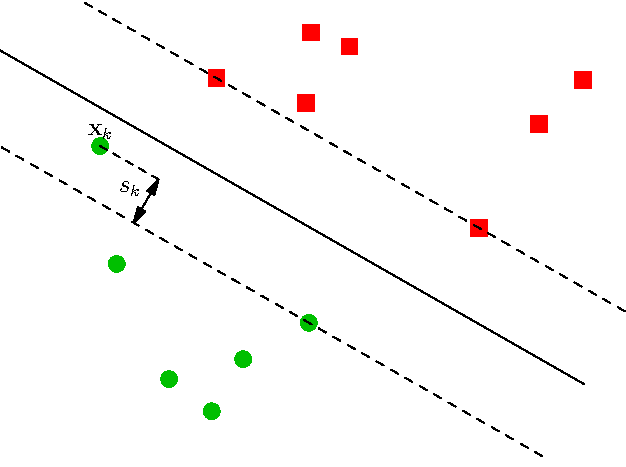
\includegraphics[width=\linewidth]{slack-variables}\pause
    \end{center}
    \end{minipage}
  \item Minimise $\frac{\|\bm{w}\|^2}{2} + C \sum_{k=1}^n s_k$\pause
  \item Large $C$ punishes slack variables\pause
  \end{itemize}
\end{PauseHighLight}

\end{slide}

%%%%%%%%%%%%%%%%%%%%%%% Next Slide %%%%%%%%%%%%%%%%%%%%%%%

\begin{slide}
\section[-2]{Dual Problem with Slack Variables}
  
\begin{PauseHighLight}
  \begin{itemize}
  \item The Lagrangian with slack variables is
    \begin{align*}
      \hspace{-2cm}\mathcal{L} = \frac{1}{2} \|\bm{w}\|^2
      + C \sum_{k=1}^m s_k
      - \sum_{k=1}^m \alpha_k \left(\strut
      y_k\,\left(\bm{w}^{\tr} \bm{\phi}(\bm{x}_k) -  b\right) - 1 + s_k
      \right) - \sum_{k=1}^m \beta_k \, s_k
    \end{align*}
    where $\beta_k$ are Lagrange multipliers that ensure $s_k\geq0$ (note
    that $\beta_k\geq0$---this is the KKT condition)\pause
  \item Now minimising with respect to $s_i$
    \begin{align*}
      \pd{\mathcal{L}}{s_i} = C - \alpha_i - \beta_i =0\pause
    \end{align*}
  \item Or $\alpha_i = C -\beta_i$.  Since $\beta_i \geq 0$ the
    constraint is $\alpha_i \leq C$\pause{} (recall also $\alpha_i\geq0$)\pauseb
  \end{itemize}
\end{PauseHighLight}

\end{slide}




%%%%%%%%%%%%%%%%%%%%%%% Next Slide %%%%%%%%%%%%%%%%%%%%%%%
\Outline % Practice
%%%%%%%%%%%%%%%%%%%%%%% Next Slide %%%%%%%%%%%%%%%%%%%%%%%

\begin{slide}
\section[-2]{Getting SVMs to Work Well}

\pb
\begin{itemize}
\item SVMs rely on distances between data points\pauseh
\item These will change relative to each other if we rescale some
  features but not other---giving different maximum-margin
  hyper-planes\pauseh
  \begin{center}
    \multipdf[width=0.3\linewidth]{rescale}\pause
  \end{center}
\item If we don't know what features are important (most often the
  case), then it is worth scaling each feature (for example, so their
  range is between 0 and 1 or their variance is 1)\pause
\end{itemize}

\end{slide}


%%%%%%%%%%%%%%%%%%%%%%% Next Slide %%%%%%%%%%%%%%%%%%%%%%%

\begin{slide}
\section[-2]{Optimising C}

\begin{PauseHighLight}
  \begin{itemize}
  \item Recall that we can introduce soft-margins using slack
    variables where we minimise
    $\frac{\|\hat{\bm{w}}\|^2}{2} + C \sum_{k=1}^m s_k$ subject to
    constraints\pause
  \item In practice it can make a huge difference to the performance if
    we change $C$\pause
  \item Optimal $C$ values changes by many orders of magnitude
    e.g. $2^{-5}$--$2^{15}$\pause
  \item Typically optimised by a grid search (start from $2^{-5}$ say and
    double until you reach $2^{15}$)\pause
  \item Measure performance on a validation set\pause
  \end{itemize}
\end{PauseHighLight}

\end{slide}

%%%%%%%%%%%%%%%%%%%%%%% Next Slide %%%%%%%%%%%%%%%%%%%%%%%

\begin{slide}
\section{Choosing the Right Kernel Function}

\begin{PauseHighLight}
  \begin{itemize}
  \item There are kernels design for particular data types (e.g. string
    kernels for text or biological sequences)\pause
  \item For numerical data people tend to look at using no kernel
    (linear SVM), a radial basis function (Gaussian) kernel or
    polynomial kernels\pause
  \item Kernel's often come with parameters, e.g. the popular radial
    basis function kernel
    \begin{align*}
       K(\bm{x},\,\bm{y}) =
      \mathrm{e}^{-\gamma\,\|\bm{x}-\bm{y}\|^2}\pause
    \end{align*}
  \item Optimal $\gamma$ values range over $2^{-15}$--$2^3$\pause
  \end{itemize}
\end{PauseHighLight}

\end{slide}

%%%%%%%%%%%%%%%%%%%%%%% Next Slide %%%%%%%%%%%%%%%%%%%%%%%

\begin{slide}
\section{Multi-Class Problems}

\begin{PauseHighLight}
  \begin{itemize}
  \item By construction SVMs separate only two classes\pause
  \item If we have a multi-class problem we have to use multiple
    SVMs\pause
  \item There are two major ways practitioners do this
    \begin{description}
    \item[One-versus-all:] for each class, train a separate classify to
      determine that class versus all others\pause
    \item[All-pairs:] train a classify for all pairs of classes\pause
    \end{description}
  \item In both cases choose the class which the classifier is most
    certain about\pause
  \end{itemize}
\end{PauseHighLight}

\end{slide}


%%%%%%%%%%%%%%%%%%%%%%% Next Slide %%%%%%%%%%%%%%%%%%%%%%%

\begin{slide}
\section{SVM Libraries}

\begin{PauseHighLight}
  \begin{itemize}
  \item Although SVMs have unique solutions, they require very well
    written optimisers\pause
  \item If you have a large data set they can be very slow\pause
  \item There are good libraries out there, svmlib, svm-lite, etc.\pause
  \item These will often automate normalisation of data and grid search
    for parameters\pause
  \end{itemize}
\end{PauseHighLight}

\end{slide}




%%%%%%%%%%%%%%%%%%%%%%% Next Slide %%%%%%%%%%%%%%%%%%%%%%%

\begin{slide}
\section{Conclusions}

\begin{PauseHighLight}
  \begin{itemize}
  \item We've seen how SVMs work\pause
  \item We've learnt how to use them\pause
  \item We've seen that we can find the maximum margin hyper-plane by
    solving a quadratic programming problem (with a unique
    solution)\pause
  \item This is a convex optimisation problem with a unique
    optimum\pause
  \item The \emph{dual problem} of an SVM is particularly simple,
    especially if we use a positive semi-definite kernel\pause{} (we
    explore these in the next lecture)\pauseb
  \end{itemize}
\end{PauseHighLight}


\end{slide}



%%% Local Variables:
%%% TeX-master: "lectures"
%%% End:
